\documentclass[conference]{IEEEtran}
\IEEEoverridecommandlockouts
\usepackage{amsmath,amssymb}
\usepackage{booktabs}
\usepackage{multirow}
\usepackage{graphicx}
\usepackage{cite}
\usepackage{url}
\usepackage{xcolor}
\usepackage{tikz}
\usetikzlibrary{arrows.meta,positioning,fit,calc}
\usepackage{stfloats}
\graphicspath{{../../../results/phase2/main/figures/}{figures/}}
\newcommand{\code}[1]{\texttt{\small #1}}

\begin{document}

\title{Multi-Cohort Heart Disease Risk Modelling: Integrating a Bayesian Network with a Regularised Neural Network under Library-Managed Hyperparameter Optimisation}

\author{
\IEEEauthorblockN{Hardik Hathwal (2401010176), Ayush (2401010121), K Akshith Kumar (2401010230),\\ Vansh Panwar (2401010494), Kabir Sharma (2401010205)}
\IEEEauthorblockA{Newton School of Technology, Rishihood University, Sonipat, India\\
Advanced Machine Learning, Phase 2 \quad Supervisor: Mr.\ Shobhit Johri}
}

\maketitle

\begin{abstract}
Phase~1 of this project compared six classical classifiers on the 303-patient Cleveland heart disease cohort. Following evaluator feedback, Phase~2 (i) uses all four independent processed cohorts of the UCI Heart Disease collection (Cleveland, Hungarian, Switzerland and Long Beach VA; 920 patients), (ii) adds a regularised multilayer perceptron (MLP), (iii) integrates the domain-structured Bayesian network (BN) with the MLP through a cross-fitted probability stack, and (iv) replaces the hand-written grid loop with library-managed Tree-structured Parzen Estimator (TPE) search through \code{OptunaSearchCV}. All eight models are evaluated under identical nested stratified cross-validation and under leave-one-cohort-out (LOCO) validation, in which each hospital is held out in turn. In pooled nested validation, discrimination is tightly clustered (ROC AUC 0.875--0.895); the MLP (0.888) and the BN--MLP stack (0.889) are statistically indistinguishable from logistic regression and the SVM, and both improve on the BN alone. Holding out a whole hospital lowers ROC AUC by 0.046--0.079 for every model; the MLP degrades most, and the stack recovers part of this loss (paired $\Delta$AUC $+0.017$, 95\% CI $[+0.005, +0.030]$ over the MLP). Ablations show that the regularisers and the second hidden layer have no measurable effect at this sample size, and SHAP analysis shows that the MLP learns smooth interactions the discretised BN cannot represent. The models are an academic comparison on historical, referral-based data and are not clinically validated.
\end{abstract}

\begin{IEEEkeywords}
Heart disease, Bayesian network, multilayer perceptron, stacking, hyperparameter optimisation, Optuna, TPE, nested cross-validation, cross-cohort validation, calibration, SHAP.
\end{IEEEkeywords}

\section{Introduction}
Coronary artery disease is commonly diagnosed by invasive angiography. Models that estimate the probability of angiographic disease from routine clinical and exercise-test variables are a long-standing benchmark problem in medical machine learning, and the UCI Heart Disease collection \cite{uci,detrano} remains one of the most widely used datasets for it.

In Phase~1 we compared six classical models --- a domain-informed Bayesian network (BN), Naive Bayes (NB), logistic regression (LR), an RBF support vector machine (SVM), random forest (RF) and gradient boosting (GB) --- on the 303-patient Cleveland cohort using 5$\times$5 repeated nested cross-validation. All six discriminated well (pooled ROC AUC 0.890--0.910) and five could not be separated statistically. The evaluator's feedback on Phase~1 set four requirements for Phase~2:
\begin{enumerate}
\item submit the report in IEEE format;
\item do not write manual loops for hyperparameter selection;
\item use all available heart disease datasets, not only Cleveland;
\item integrate the existing machine-learning (ML) work with a deep-learning (DL) component and use an advanced hyperparameter-selection method.
\end{enumerate}
This paper documents how Phase~2 meets each requirement and what the results show. We address four research questions:
\begin{itemize}
\item \textbf{RQ1.} Does a regularised MLP improve on the Phase~1 models when all four cohorts are pooled?
\item \textbf{RQ2.} Does a leakage-safe integration of the BN and the MLP outperform either constituent?
\item \textbf{RQ3.} How much does performance fall when the model must generalise to a hospital it has never seen?
\item \textbf{RQ4.} Which architectural and regularisation choices of the MLP actually matter at this sample size?
\end{itemize}
Our contributions are: a 920-patient, four-cohort data audit with provenance and hashes; a scikit-learn-compatible PyTorch MLP whose preprocessing and early stopping never see held-out rows; a cross-fitted BN--MLP stack; TPE-based selection of every hyperparameter through \code{OptunaSearchCV}, with saved trial histories; two complementary validation protocols with patient-level bootstrap intervals and paired comparisons; and controlled ablations and SHAP attributions. The code, tests and every number in this paper are traceable to one saved run (\code{results/phase2/main}).

\section{Related Work}
\subsection{Heart disease prediction}
The four cohorts were collected by Detrano \textit{et al.} \cite{detrano}, who derived a probability algorithm in Cleveland and then applied it to the Hungarian, Swiss and VA populations --- an early example of cross-site validation that motivates our LOCO protocol. Most later studies use only the Cleveland subset and report a single random split, which makes their results hard to compare; we follow the guidance of TRIPOD \cite{tripod} and Steyerberg \cite{steyerberg} in reporting calibration as well as discrimination and in separating internal from cross-site validation.

\subsection{Probabilistic graphical models}
Bayesian networks encode a joint distribution as a directed acyclic graph with conditional probability tables (CPTs) \cite{pearl,koller}. BN classifiers generalise NB by relaxing its independence assumption \cite{friedman_bnc}. Our BN uses an expert-specified structure and learns only Dirichlet-smoothed CPTs with \code{pgmpy} \cite{pgmpy}.

\subsection{Deep learning on small tabular data}
Feed-forward networks are universal approximators \cite{goodfellow}, but large benchmarks show that on medium-sized tabular data tree ensembles and well-tuned linear models are usually as good or better \cite{grinsztajn,shwartz}; a carefully regularised MLP is nonetheless a strong baseline \cite{gorishniy}. Dropout \cite{dropout}, weight decay \cite{adamw}, early stopping \cite{prechelt} and Adam \cite{adam} are the standard means of controlling capacity. Convolutional or recurrent layers have no natural inductive bias for unordered patient features, so we deliberately did not use them.

\subsection{Hyperparameter optimisation}
Grid search scales exponentially with the number of hyperparameters; random search is more efficient \cite{bergstra_random}, and sequential model-based methods such as Gaussian-process Bayesian optimisation \cite{snoek} and TPE \cite{bergstra} use earlier trials to choose later ones. Optuna \cite{optuna} implements TPE with a define-by-run API and an scikit-learn-compatible \code{OptunaSearchCV} estimator. Selection must be nested inside the evaluation loop, otherwise performance is optimistically biased \cite{varma,cawley}.

\subsection{Model integration, calibration and explanation}
Stacked generalisation trains a meta-learner on out-of-fold base predictions \cite{wolpert,breiman_stack,superlearner}; training it on in-sample predictions leaks information. Calibration of probabilistic classifiers \cite{niculescu,guo} matters when outputs are read as risks. SHAP \cite{shap} attributes a prediction to its inputs using Shapley values. Performance under hospital change is a form of dataset shift \cite{datasetshift}.

\section{Data}
\subsection{Cohorts and target}
We use exactly the four processed files of the UCI archive (Table~\ref{tab:cohorts}). The raw and \code{reprocessed.hungarian} files are alternative encodings of the same patients and are excluded, so no patient appears twice. Each file's SHA-256 hash, the archive hash and per-cohort counts are recorded in \code{data\_verification.json}. A \code{cohort} column is kept for provenance, grouping and reporting but is never a predictor. The target keeps the Phase~1 definition: \code{num}$\,=0 \rightarrow 0$ (no $\geq$50\% stenosis) and \code{num}$\,\in\{1,\dots,4\} \rightarrow 1$.

\begin{table}[t]
\caption{The four processed UCI cohorts used in Phase~2}
\label{tab:cohorts}
\centering
\footnotesize
\setlength{\tabcolsep}{4pt}
\begin{tabular}{lrrrrr}
\toprule
Cohort & Patients & Disease & Healthy & Prevalence & Missing cells \\
\midrule
Cleveland & 303 & 139 & 164 & 45.9\% & 6 \\
Hungarian & 294 & 106 & 188 & 36.1\% & 782 \\
Switzerland & 123 & 115 & 8 & 93.5\% & 273 \\
Long Beach VA & 200 & 149 & 51 & 74.5\% & 698 \\
\midrule
Total & 920 & 509 & 411 & 55.3\% & 1759 \\
\bottomrule
\end{tabular}
\end{table}

\subsection{Predictors and missingness}
The 13 predictors are age, sex, chest pain type (\code{cp}), resting blood pressure (\code{trestbps}), cholesterol (\code{chol}), fasting blood sugar (\code{fbs}), resting ECG (\code{restecg}), maximum heart rate (\code{thalach}), exercise angina (\code{exang}), ST depression (\code{oldpeak}), ST slope (\code{slope}), number of fluoroscopy-coloured vessels (\code{ca}) and thallium scan result (\code{thal}). Figure~\ref{fig:audit} summarises the audit. Missingness is severe and strongly cohort-structured: \code{ca} is missing for 611 of 920 patients (66.4\%), \code{thal} for 486 (52.8\%) and \code{slope} for 309 (33.6\%), but almost never in Cleveland. Because the missing pattern is determined by the hospital rather than by chance, the data are not missing completely at random \cite{little}, and complete-case analysis would discard most non-Cleveland patients. We therefore impute inside every training fold (Section~\ref{sec:prep}). Prevalence also differs sharply between cohorts (36\%--94\%); Switzerland has only eight disease-free patients, so its specificity and per-cohort AUC are very uncertain. The audit flagged one exact duplicate feature row in each of Hungarian and VA; both were retained because identical measurements can belong to different patients and patient identifiers are unique.

\begin{figure}[t]
\centering
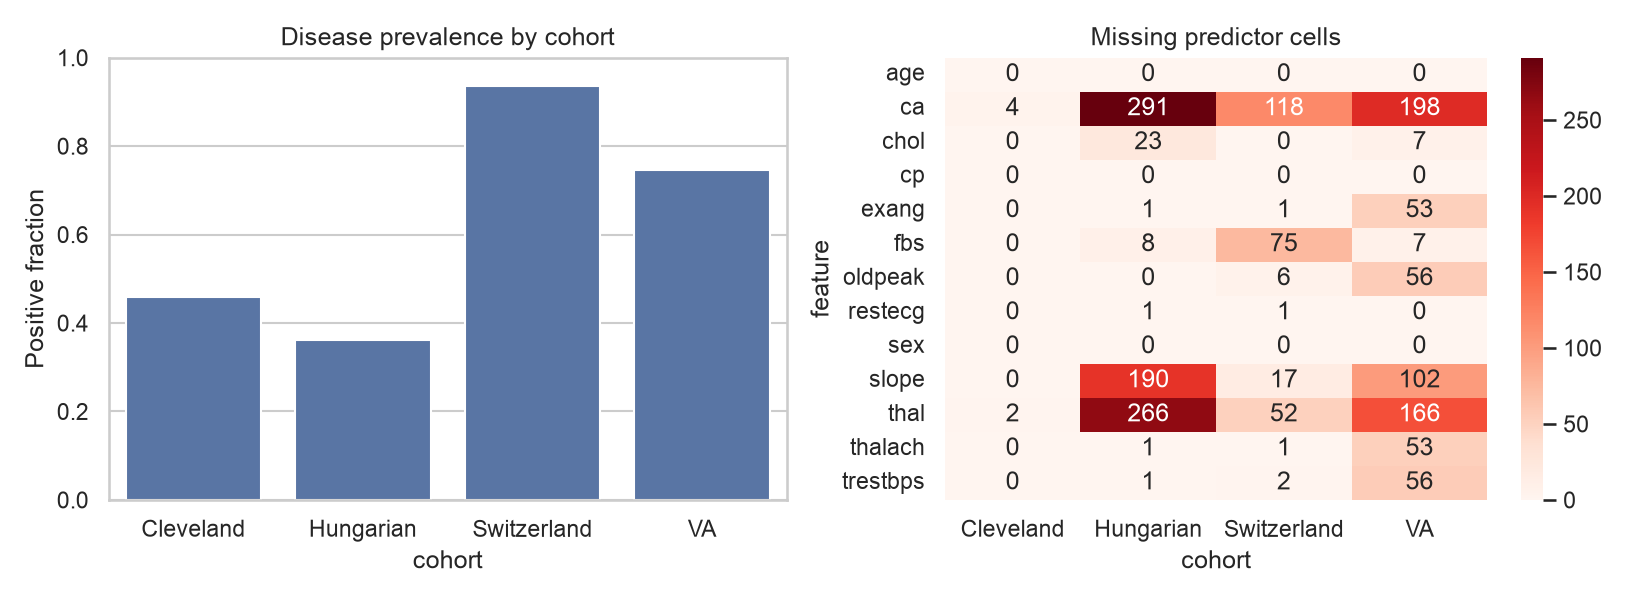
\includegraphics[width=\columnwidth]{cohort_data_audit.png}
\caption{Four-cohort audit: disease prevalence (left) and missing predictor cells (right) by cohort.}
\label{fig:audit}
\end{figure}

\section{Methods}
\subsection{Preprocessing and leakage controls}\label{sec:prep}
Every data-dependent transformation is part of the estimator and is re-fitted on the training rows of each fold. A guard rejects the target columns as predictors. Two pipelines from Phase~1 are reused:
\begin{itemize}
\item \textit{Numeric} (LR, SVM, RF, GB, MLP): median imputation and standardisation of the five continuous features, most-frequent imputation of binary features, most-frequent imputation and standardisation of the ordinal \code{ca} and \code{slope}, and most-frequent imputation plus one-hot encoding of \code{cp}, \code{restecg} and \code{thal}. This yields 20 inputs.
\item \textit{Discrete} (BN, NB): continuous features cut into training-fold tertiles; missing or unseen values mapped to the training-fold mode; 13 integer-coded variables.
\end{itemize}
\textit{BN missing-data decision.} The BN could treat ``missing'' as an extra state of each node, but because missingness is almost entirely determined by cohort, that state would act as a hospital indicator and let the BN learn cohort prevalence rather than disease mechanism, which would also break LOCO validation. We therefore impute the training-fold mode inside each fold and accept the resulting loss of information as a documented limitation.

\subsection{Classical reference models}
The six Phase~1 models are retained unchanged apart from their search spaces: the BN with the Phase~1 expert DAG of 14 nodes and 16 edges and exact variable-elimination inference \cite{pearl,pgmpy}; categorical NB; L2-regularised LR; an RBF SVM \cite{cortes} with Platt scaling \cite{platt}; RF \cite{breiman_rf}; and GB \cite{friedman_gb}, all from scikit-learn \cite{sklearn}.

\subsection{Regularised MLP}
The MLP (\code{TabularMLPClassifier}, PyTorch \cite{pytorch}) maps the transformed input $\mathbf{x}\in\mathbb{R}^{d}$ ($d=20$, inferred at fit time rather than hard-coded) through $L\in\{1,2\}$ hidden layers:
\begin{equation}
\mathbf{h}^{(l)} = \operatorname{Dropout}_p\!\big(\operatorname{ReLU}(\mathbf{W}^{(l)}\mathbf{h}^{(l-1)} + \mathbf{b}^{(l)})\big),\qquad \mathbf{h}^{(0)}=\mathbf{x},
\end{equation}
\begin{equation}
\hat{p} = \sigma\big(\mathbf{w}^{\top}\mathbf{h}^{(L)} + b\big).
\end{equation}
Weights are fitted by mini-batch Adam \cite{adam} on the binary cross-entropy with an L2 penalty:
\begin{equation}
\mathcal{L} = -\frac{1}{n}\sum_{i=1}^{n}\big[y_i\log\hat{p}_i + (1-y_i)\log(1-\hat{p}_i)\big] + \frac{\lambda}{2}\lVert\boldsymbol\theta\rVert_2^2 .
\end{equation}
(PyTorch's \code{Adam(weight\_decay)} adds $\lambda\boldsymbol\theta$ to the gradient, i.e.\ coupled L2 regularisation rather than the decoupled AdamW form \cite{adamw}.) Early stopping \cite{prechelt} is made leakage-safe: inside \code{fit}, the \emph{raw} training rows are first split 80/20 (stratified) into weight-training and stopping rows; the preprocessor is fitted on the 80\% only; training stops when stopping-set loss has not improved by $10^{-4}$ for 15 epochs (maximum 150), and the best weights are restored. Outer-test patients therefore influence neither preprocessing, nor weights, nor the stopping epoch.

The search space (Table~\ref{tab:space}) allows three layouts: 16 (353 parameters), 16--8 (481) and 32--16 (1{,}217). Even the largest has only about two parameters per weight-training patient ($\approx$590 per fold), and dropout, weight decay and early stopping further limit its effective capacity. Fig.~\ref{fig:arch} shows the architecture.

\begin{figure}[t]
\centering
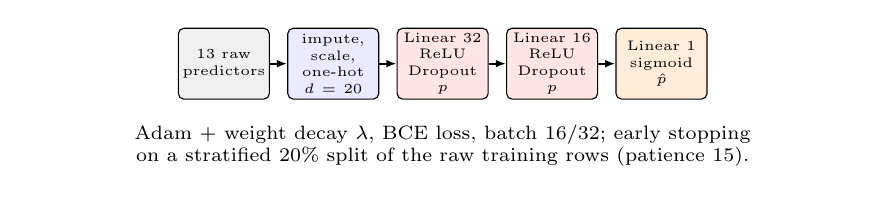
\begin{tikzpicture}[font=\tiny, node distance=2.2mm,
  box/.style={draw, rounded corners=2pt, align=center, text width=10.5mm, minimum height=9mm, inner sep=1.5pt},
  arr/.style={-{Latex[length=1.3mm]}, thick}]
\node[box, fill=gray!12] (raw) {13 raw\\predictors};
\node[box, fill=blue!8, right=of raw] (pre) {impute,\\scale,\\one-hot\\$d=20$};
\node[box, fill=red!10, right=of pre] (h1) {Linear 32\\ReLU\\Dropout $p$};
\node[box, fill=red!10, right=of h1] (h2) {Linear 16\\ReLU\\Dropout $p$};
\node[box, fill=orange!15, right=of h2] (out) {Linear 1\\sigmoid\\$\hat p$};
\draw[arr] (raw) -- (pre); \draw[arr] (pre) -- (h1); \draw[arr] (h1) -- (h2); \draw[arr] (h2) -- (out);
\node[anchor=north, align=center, text width=0.85\columnwidth, font=\scriptsize] at ($(raw.south)!0.5!(out.south)+(0,-2mm)$)
 {Adam + weight decay $\lambda$, BCE loss, batch 16/32; early stopping on a stratified 20\% split of the raw training rows (patience 15).};
\end{tikzpicture}
\caption{The 32--16 MLP layout (selected in four of five pooled outer folds). The preprocessor is fitted only on the weight-training rows.}
\label{fig:arch}
\end{figure}

\subsection{BN--MLP integration by cross-fitted stacking}
The BN and the MLP make different assumptions: the BN imposes clinical structure, gives calibrated probabilities through explicit CPTs and transfers well, while the MLP models smooth nonlinear interactions on continuous inputs. We integrate them with a stacked generalisation \cite{wolpert,superlearner} (\code{BNMLPStackingClassifier}). Given a training set $D$:
\begin{enumerate}
\item split $D$ into $K=3$ stratified folds; for each fold $k$, fit the BN and the MLP on $D\setminus D_k$ and predict $D_k$, giving out-of-fold probabilities $\big(p^{\text{BN}}_i, p^{\text{MLP}}_i\big)$ for every training patient;
\item fit a regularised logistic combiner $\hat p_i = \sigma(\beta_0 + \beta_1 p^{\text{BN}}_i + \beta_2 p^{\text{MLP}}_i)$ with inverse strength $C$;
\item refit the BN and the MLP on all of $D$; at prediction time their probabilities feed the combiner.
\end{enumerate}
Each meta-feature therefore comes from a base model that never saw that patient, and the whole procedure runs inside the outer training fold, so outer patients never reach it. A unit test checks the cross-fitting property. As an integration control, \code{BNMLPAverageClassifier} averages the two probabilities without learning.

\subsection{Library-managed hyperparameter selection}
Phase~1 enumerated a grid with a hand-written \code{for params in combos} loop. Phase~2 removes this: one shared builder (\code{make\_search}) wraps each model in \code{optuna\_integration.OptunaSearchCV} with a seeded \code{TPESampler}, a stratified 3-fold inner CV, \code{scoring="neg\_log\_loss"}, 12 trials and \code{refit=True}. TPE models the density of good configurations $\ell(\mathbf{x})$ and of the rest $g(\mathbf{x})$ and proposes the candidate that maximises $\ell(\mathbf{x})/g(\mathbf{x})$ \cite{bergstra}, so later trials concentrate where earlier ones did well. Log loss is used because it rewards calibrated probabilities, not just ranking. Table~\ref{tab:space} lists the search spaces, which were frozen before the main run; log-uniform priors are used for scale parameters. The library owns all candidate iteration and inner cross-validation; the only project loops iterate over outer folds and models, which is evaluation, not selection. Each outer fold uses seed $42+k$, and \code{best\_params\_}, \code{best\_score\_}, runtime and the full trial history (480 pooled and 384 LOCO trials) are saved.

\begin{table}[t]
\caption{TPE search spaces (12 trials per outer fold)}
\label{tab:space}
\centering
\scriptsize
\begin{tabular}{p{0.17\columnwidth}p{0.73\columnwidth}}
\toprule
Model & Hyperparameters and ranges \\
\midrule
BN & pseudo-count $\in[0.5, 50]$ (log) \\
NB & $\alpha\in[0.5, 50]$ (log) \\
LR & $C\in[0.01, 10]$ (log) \\
SVM & $C\in[0.1, 10]$ (log); $\gamma\in\{\text{scale}, 0.01, 0.1\}$ \\
RF & trees $\in\{100,\dots,400\}$; depth $\in\{3,5,\text{None}\}$; min leaf $\in\{1,\dots,4\}$ \\
GB & learning rate $\in[0.02,0.2]$ (log); trees $\in\{50,\dots,200\}$; depth $\in\{1,2,3\}$ \\
MLP & layout $\in\{16, 16\text{--}8, 32\text{--}16\}$; dropout $\in[0.1,0.5]$; lr $\in[10^{-4}, 3\cdot10^{-3}]$ (log); weight decay $\in[10^{-5},10^{-2}]$ (log); batch $\in\{16,32\}$ \\
Stack & BN pseudo-count; MLP layout, dropout, lr, weight decay (as above); meta $C\in[0.01,10]$ (log) \\
\bottomrule
\end{tabular}
\end{table}

\subsection{Evaluation protocols}
Fig.~\ref{fig:protocol} shows the two protocols.

\textit{Pooled nested CV (primary).} Five stratified outer folds over all 920 patients (seed 42). In each, \code{OptunaSearchCV} selects and refits on the outer training rows, and the outer test rows are scored once. Every model sees the same outer folds (fold hash \code{2932cad8231cce43}).

\textit{Leave-one-cohort-out (LOCO).} Scikit-learn's \code{LeaveOneGroupOut} with \code{cohort} as the group: train (including the full TPE search) on three hospitals and test on the fourth. This measures transfer to an unseen site, as in the original multi-centre study \cite{detrano}. It is cross-cohort validation of historical data, not prospective clinical validation.

\begin{figure}[t]
\centering
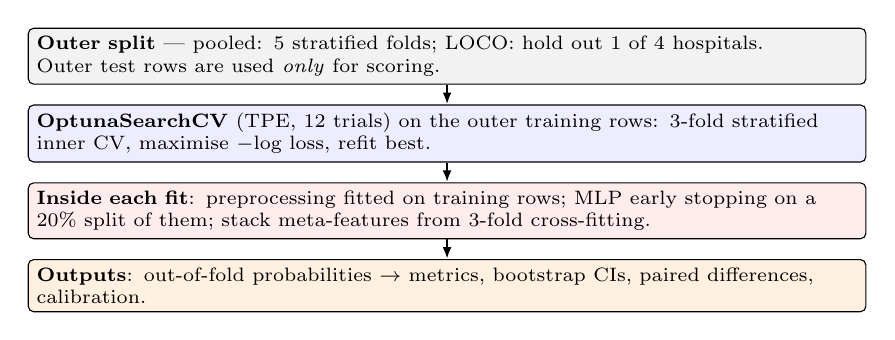
\begin{tikzpicture}[font=\scriptsize,
  lvl/.style={draw, rounded corners=2pt, align=left, text width=0.86\columnwidth, inner sep=3pt},
  arr/.style={-{Latex[length=1.5mm]}, thick}]
\node[lvl, fill=gray!10] (o) {\textbf{Outer split} --- pooled: 5 stratified folds; LOCO: hold out 1 of 4 hospitals.\\ Outer test rows are used \emph{only} for scoring.};
\node[lvl, fill=blue!7, below=2.5mm of o] (i) {\textbf{OptunaSearchCV} (TPE, 12 trials) on the outer training rows: 3-fold stratified inner CV, maximise $-$log loss, refit best.};
\node[lvl, fill=red!7, below=2.5mm of i] (m) {\textbf{Inside each fit}: preprocessing fitted on training rows; MLP early stopping on a 20\% split of them; stack meta-features from 3-fold cross-fitting.};
\node[lvl, fill=orange!12, below=2.5mm of m] (r) {\textbf{Outputs}: out-of-fold probabilities $\rightarrow$ metrics, bootstrap CIs, paired differences, calibration.};
\draw[arr] (o) -- (i); \draw[arr] (i) -- (m); \draw[arr] (m) -- (r);
\end{tikzpicture}
\caption{Nested evaluation design. No outer-test patient affects preprocessing, hyperparameters, early stopping, stacking or the 0.5 threshold.}
\label{fig:protocol}
\end{figure}

\textit{Metrics.} From the out-of-fold probabilities we report ROC AUC, PR AUC, Brier score, log loss, expected calibration error (ECE, 10 bins), and accuracy, sensitivity and specificity at the pre-registered threshold 0.5. Results are given overall and per cohort.

\textit{Uncertainty.} 95\% percentile intervals come from 500 patient-level bootstrap resamples \cite{efron}. Paired differences between models use 2{,}000 bootstrap resamples in which both models are scored on the same resampled patients; an interval excluding zero is marked $^{*}$. With eight model pairs and three metrics per protocol this is modest evidence, and we do not correct for multiplicity.

\subsection{Ablations and explanation}
Ablations use fixed, non-searched settings (MLP 16--8, dropout 0.3, weight decay $10^{-3}$, lr $10^{-3}$, batch 32; BN pseudo-count 2) and 5-fold stratified \code{cross\_validate}, changing one factor at a time: no dropout, no weight decay, no early stopping (150 epochs), and one hidden layer. The integration ablation compares BN alone, MLP alone, the simple average and the learned stack. These are controlled comparisons, not hyperparameter candidates. For explanation, KernelSHAP \cite{shap} is applied to the MLP fitted on all 920 patients (250 complete-case explained patients, 40 background rows, 150 coalition samples), and the learned MLP and BN risk surfaces are plotted over pairs of predictors.

\subsection{Software and reproducibility}
Python 3.11.16, NumPy 2.4.6, pandas 2.3.3, scikit-learn 1.9.1, PyTorch 2.15.0, Optuna 5.1.0 and pgmpy; one project seed (42) controls all splits, searches and networks. Each run writes a manifest with file hashes, cohort counts, fold hashes, versions and search settings. Tests cover data loading and counts, MLP fitting, cloning and reproducibility, search-space validity, the cross-fitting property and the saved artifacts. Phase~1 code, configuration and results are kept unchanged beside the Phase~2 files.

\section{Results}
\subsection{Pooled nested validation (RQ1, RQ2)}
Table~\ref{tab:pooled} and Fig.~\ref{fig:curves} report the primary results. All eight models discriminate well and are tightly clustered: ROC AUC ranges from 0.875 (BN) to 0.895 (SVM), and the per-fold standard deviation is 0.015--0.028. The MLP reaches 0.888 and the stack 0.889. Both are among the best calibrated models (ECE 0.018 and 0.023; calibration curves lie close to the diagonal).

\begin{table*}[t]
\caption{Pooled nested cross-validation on 920 patients (5 outer folds; threshold 0.5). Best value per column in bold.}
\label{tab:pooled}
\centering
\footnotesize
\begin{tabular}{lcccccccc}
\toprule
Model & ROC AUC [95\% CI] & PR AUC & Brier & Log loss & ECE & Acc. & Sens. & Spec. \\
\midrule
BN & 0.875 [0.851, 0.896] & 0.884 & 0.142 & 0.449 & 0.045 & 0.801 & 0.813 & 0.786 \\
NB & 0.879 [0.854, 0.900] & 0.881 & 0.139 & 0.444 & 0.035 & 0.809 & 0.829 & 0.783 \\
LR & 0.889 [0.866, 0.909] & \textbf{0.896} & 0.131 & 0.417 & 0.028 & 0.824 & 0.857 & 0.783 \\
SVM & \textbf{0.895} [0.874, 0.916] & 0.893 & \textbf{0.126} & \textbf{0.405} & 0.020 & 0.817 & 0.870 & 0.752 \\
RF & 0.886 [0.863, 0.908] & 0.884 & 0.133 & 0.422 & 0.035 & 0.811 & 0.855 & 0.757 \\
GB & 0.889 [0.868, 0.910] & 0.890 & 0.131 & 0.416 & 0.030 & 0.810 & 0.851 & 0.759 \\
\midrule
MLP & 0.888 [0.865, 0.909] & 0.889 & 0.131 & 0.418 & \textbf{0.018} & 0.818 & 0.841 & 0.791 \\
BN--MLP stack & 0.889 [0.864, 0.909] & 0.893 & 0.129 & 0.414 & 0.023 & 0.822 & 0.862 & 0.771 \\
\bottomrule
\end{tabular}

\end{table*}

\begin{figure}[t]
\centering
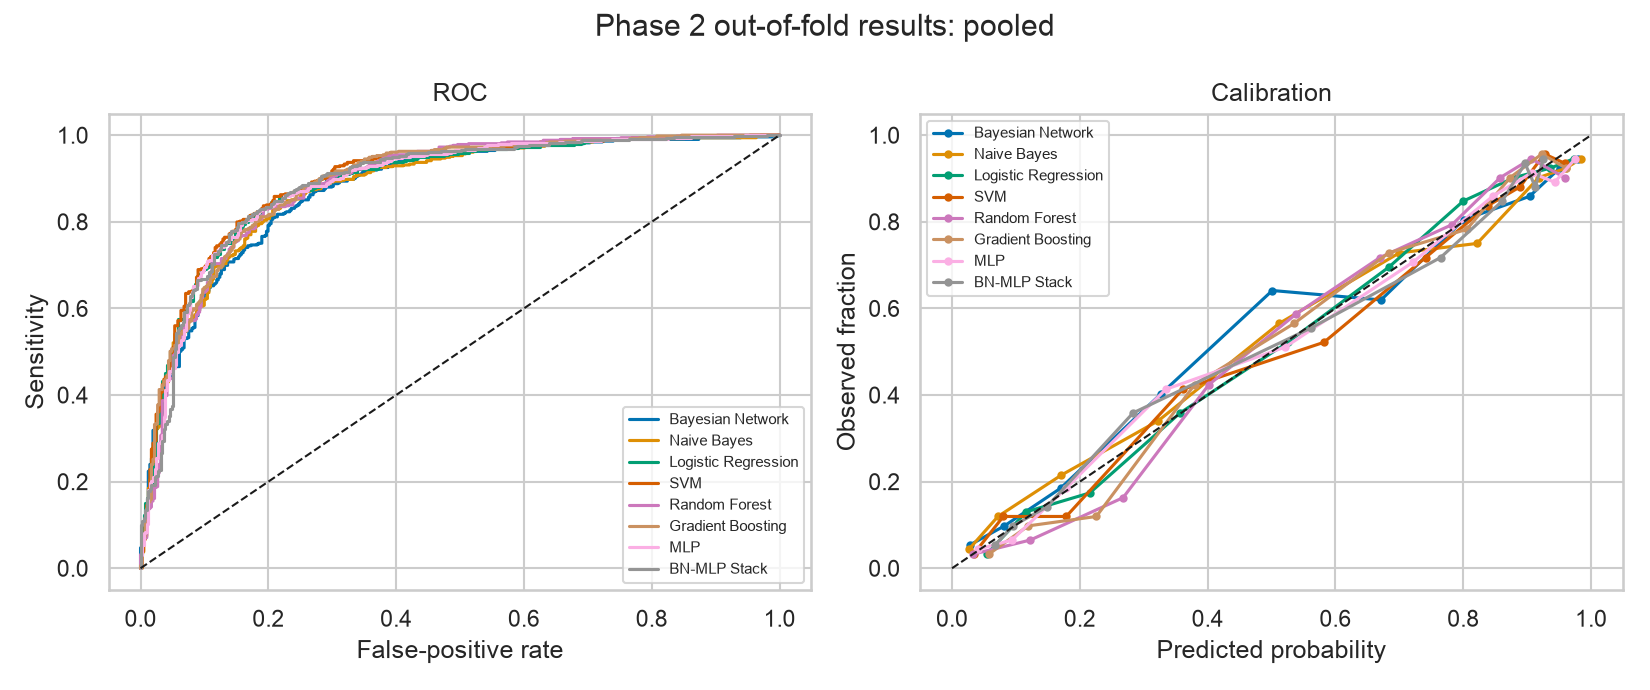
\includegraphics[width=\columnwidth]{curves_pooled.png}
\caption{Pooled out-of-fold ROC curves (left) and quantile reliability curves (right) for all eight models.}
\label{fig:curves}
\end{figure}

The paired comparisons (Table~\ref{tab:paired}) answer RQ1 and RQ2. The MLP is indistinguishable from LR ($-0.001$) and from the SVM ($-0.007$, interval includes zero), so on pooled data a neural network adds no discrimination over the best Phase~1 models. The MLP does improve on the BN ($+0.013$, $^{*}$), and the stack improves on the BN ($+0.014$, $^{*}$) but not on the MLP ($+0.001$). The stack's log loss (0.414) and Brier score (0.129) are slightly better than those of the MLP (0.418, 0.131), but these differences are also within noise. In short, under random patient splits the integrated model is as good as its best constituent and as good as the strongest classical models, but not better.

\begin{table}[t]
\caption{Paired bootstrap differences in ROC AUC (2{,}000 resamples). $^{*}$ = 95\% interval excludes zero}
\label{tab:paired}
\centering
\scriptsize
\setlength{\tabcolsep}{3pt}
\begin{tabular}{lcc}
\toprule
Comparison ($A-B$) & Pooled $\Delta$AUC [95\% CI] & LOCO $\Delta$AUC [95\% CI] \\
\midrule
BN--MLP stack $-$ MLP & $+0.001$ [$-0.006$, $+0.007$] & $+0.017$ [$+0.005$, $+0.030$]$^{*}$ \\
BN--MLP stack $-$ BN & $+0.014$ [$+0.004$, $+0.024$]$^{*}$ & $+0.008$ [$-0.003$, $+0.020$] \\
MLP $-$ BN & $+0.013$ [$+0.001$, $+0.025$]$^{*}$ & $-0.009$ [$-0.028$, $+0.010$] \\
MLP $-$ LR & $-0.001$ [$-0.009$, $+0.006$] & $-0.018$ [$-0.031$, $-0.005$]$^{*}$ \\
MLP $-$ SVM & $-0.007$ [$-0.017$, $+0.002$] & $-0.016$ [$-0.034$, $+0.001$] \\
BN--MLP stack $-$ SVM & $-0.007$ [$-0.016$, $+0.003$] & $+0.000$ [$-0.019$, $+0.018$] \\
SVM $-$ BN & $+0.020$ [$+0.009$, $+0.032$]$^{*}$ & $+0.007$ [$-0.015$, $+0.031$] \\
LR $-$ BN & $+0.014$ [$+0.006$, $+0.024$]$^{*}$ & $+0.010$ [$-0.003$, $+0.022$] \\
\bottomrule
\end{tabular}

\end{table}

\subsection{Generalisation to an unseen hospital (RQ3)}
Table~\ref{tab:shift} contrasts the two protocols, and Table~\ref{tab:cohort} breaks AUC down by cohort. Every model loses discrimination when the test hospital is absent from training: ROC AUC on the concatenated LOCO predictions falls by 0.046--0.079, and the mean of the four held-out-cohort AUCs is 0.769--0.810. The ranking also changes. The simplest probabilistic models transfer best (NB 0.810, BN 0.804 mean held-out AUC), whereas the most flexible models, the MLP (0.769) and the SVM (0.788), degrade most. Here the integration helps: the stack beats the MLP alone by $+0.017$ ROC AUC (95\% CI $[+0.005,+0.030]$) and by 0.030 in log loss, while under pooled CV the two were tied. The BN component appears to stabilise the MLP under hospital shift. Under LOCO, the MLP is also significantly worse than LR ($-0.018$, $^{*}$).

\begin{table}[t]
\caption{ROC AUC under pooled CV vs.\ leave-one-cohort-out}
\label{tab:shift}
\centering
\scriptsize
\setlength{\tabcolsep}{3pt}
\begin{tabular}{lcccc}
\toprule
Model & Pooled AUC & LOCO AUC & Mean held-out AUC & $\Delta$ (LOCO$-$pooled) \\
\midrule
BN & 0.875 & 0.817 & 0.804 & $-0.057$ \\
NB & 0.879 & 0.832 & \textbf{0.810} & $-0.046$ \\
LR & 0.889 & 0.827 & 0.783 & $-0.062$ \\
SVM & 0.895 & 0.825 & 0.788 & $-0.070$ \\
RF & 0.886 & 0.827 & 0.800 & $-0.059$ \\
GB & 0.889 & 0.825 & 0.792 & $-0.064$ \\
\midrule
MLP & 0.888 & 0.809 & 0.769 & $-0.079$ \\
BN--MLP stack & 0.889 & 0.825 & 0.783 & $-0.063$ \\
\bottomrule
\end{tabular}

\end{table}

\begin{table*}[t]
\caption{ROC AUC by cohort. Left: pooled nested CV predictions split by cohort. Right: each cohort held out entirely (LOCO).}
\label{tab:cohort}
\centering
\footnotesize
\begin{tabular}{lcccccccc}
\toprule
 & \multicolumn{4}{c}{Pooled nested CV (by cohort)} & \multicolumn{4}{c}{Held-out cohort (LOCO)} \\
\cmidrule(lr){2-5}\cmidrule(lr){6-9}
Model & Cle & Hun & Swi & VA & Cle & Hun & Swi & VA \\
\midrule
BN & 0.878 & 0.899 & 0.777 & 0.728 & 0.851 & 0.878 & 0.766 & 0.719 \\
NB & 0.879 & 0.892 & 0.759 & 0.745 & 0.858 & 0.886 & 0.759 & 0.736 \\
LR & 0.897 & 0.889 & 0.714 & 0.734 & 0.828 & 0.873 & 0.721 & 0.709 \\
SVM & 0.894 & 0.899 & 0.747 & 0.727 & 0.820 & 0.877 & 0.774 & 0.680 \\
RF & 0.896 & 0.887 & 0.766 & 0.693 & 0.856 & 0.881 & 0.775 & 0.686 \\
GB & 0.893 & 0.891 & 0.695 & 0.699 & 0.858 & 0.871 & 0.762 & 0.677 \\
\midrule
MLP & 0.891 & 0.888 & 0.777 & 0.702 & 0.841 & 0.851 & 0.709 & 0.674 \\
BN--MLP stack & 0.889 & 0.893 & 0.740 & 0.720 & 0.828 & 0.878 & 0.726 & 0.702 \\
\bottomrule
\end{tabular}

\end{table*}

The per-cohort results show two separate effects. First, the VA and Switzerland cohorts are hard even when patients from the same hospital are in training (pooled-CV AUC 0.69--0.78), because their high prevalence, heavy missingness of \code{ca}, \code{thal} and \code{slope}, and small numbers of healthy patients leave little signal. Second, holding a cohort out lowers AUC further, most for Cleveland, the only cohort with complete \code{ca} and \code{thal}: the other three hospitals provide almost no information about these two strongest predictors, so models trained without Cleveland cannot exploit them. Full LOCO metrics (Table~\ref{tab:cross}) also show poorer calibration (ECE up to 0.067) because each test hospital's prevalence differs from the training mixture; specificity on Switzerland rests on eight patients and should not be interpreted.

\begin{table*}[t]
\caption{Leave-one-cohort-out validation: metrics on the concatenated held-out predictions of all four folds (920 patients)}
\label{tab:cross}
\centering
\footnotesize
\begin{tabular}{lcccccccc}
\toprule
Model & ROC AUC [95\% CI] & PR AUC & Brier & Log loss & ECE & Acc. & Sens. & Spec. \\
\midrule
BN & 0.817 [0.790, 0.844] & 0.845 & 0.175 & 0.528 & 0.045 & 0.743 & 0.782 & 0.696 \\
NB & \textbf{0.832} [0.805, 0.858] & \textbf{0.850} & 0.167 & 0.513 & 0.048 & 0.757 & 0.786 & 0.720 \\
LR & 0.827 [0.799, 0.855] & 0.840 & 0.169 & 0.514 & 0.041 & 0.743 & 0.737 & 0.752 \\
SVM & 0.825 [0.797, 0.853] & 0.824 & \textbf{0.164} & \textbf{0.506} & 0.048 & 0.771 & 0.833 & 0.693 \\
RF & 0.827 [0.801, 0.854] & 0.825 & 0.168 & 0.515 & \textbf{0.038} & 0.757 & 0.778 & 0.730 \\
GB & 0.825 [0.796, 0.851] & 0.825 & 0.172 & 0.529 & 0.067 & 0.754 & 0.713 & 0.805 \\
\midrule
MLP & 0.809 [0.778, 0.838] & 0.808 & 0.177 & 0.552 & 0.064 & 0.745 & 0.756 & 0.730 \\
BN--MLP stack & 0.825 [0.796, 0.853] & 0.824 & 0.172 & 0.521 & 0.059 & 0.754 & 0.766 & 0.740 \\
\bottomrule
\end{tabular}

\end{table*}

\subsection{Hyperparameter-search evidence}
Table~\ref{tab:search} summarises the TPE selections across the five pooled outer folds. Two observations follow. First, widening the BN pseudo-count range to $[0.5,50]$ resolved a Phase~1 limitation: in Phase~1 the BN chose the top grid value (10) in all 25 folds, whereas now it chose interior values (15.4--28.8). NB's $\alpha$ (43.6--49.9) is still close to the upper bound of 50, which indicates that heavy smoothing suits the larger, noisier data, and the range should be widened further. Second, the MLP chose the 32--16 layout in four of five folds with moderate dropout (0.20--0.41) and batch size 16 in four folds; selected weight decay varied over three orders of magnitude, consistent with the ablation finding that it barely matters. In the pooled protocol, search was cheap for the classical models (2--27\,s in total) and dominated by the MLP (72\,s) and the stack (211\,s), whose cost multiplies inner folds, stacking folds and trials.

\begin{table}[t]
\caption{Hyperparameters chosen by TPE in the 5 pooled outer folds}
\label{tab:search}
\centering
\scriptsize
\setlength{\tabcolsep}{3pt}
\begin{tabular}{p{0.16\linewidth}p{0.62\linewidth}r}
\toprule
Model & Selected values over the 5 pooled outer folds & Time (s) \\
\midrule
BN & pseudo\_count 15.4--28.8 & 12 \\
NB & alpha 43.6--49.9 & 2 \\
LR & C 0.154--0.467 & 3 \\
SVM & C 0.451--6.69; gamma scale(3), 0.1(1), 0.01(1) & 6 \\
RF & max\_depth None(5); min\_samples\_leaf 2(3), 3(1), 1(1); n\_estimators 200(2), 400(1), 300(1), 100(1) & 27 \\
GB & learning\_rate 0.0363--0.122; max\_depth 1(2), 2(2), 3(1); n\_estimators 200(2), 150(2), 100(1) & 12 \\
MLP & batch\_size 16(4), 32(1); dropout 0.202--0.41; hidden\_layout 32-16(4), 16(1); learning\_rate 0.00047--0.00263; weight\_decay 1.17e-05--0.00877 & 72 \\
BN--MLP stack & bn\_pseudo\_count 0.542--7.43; meta\_C 1.01--8.01; mlp\_dropout 0.109--0.453; mlp\_hidden\_layout 32-16(2), 16(2), 16-8(1); mlp\_learning\_rate 0.000258--0.00294; mlp\_weight\_decay 1.4e-05--0.000581 & 211 \\
\bottomrule
\end{tabular}

\end{table}

\subsection{MLP training dynamics}
Fig.~\ref{fig:lc} shows the training and stopping-set losses for the MLP selected in pooled outer fold~0 (32--16 layout, 1{,}217 parameters, 588 weight-training and 148 stopping rows). The stopping loss levels off after about 20 epochs while the training loss keeps falling; early stopping restored the epoch-40 weights after 55 epochs. The widening gap is the expected sign of the onset of overfitting.

\begin{figure}[t]
\centering
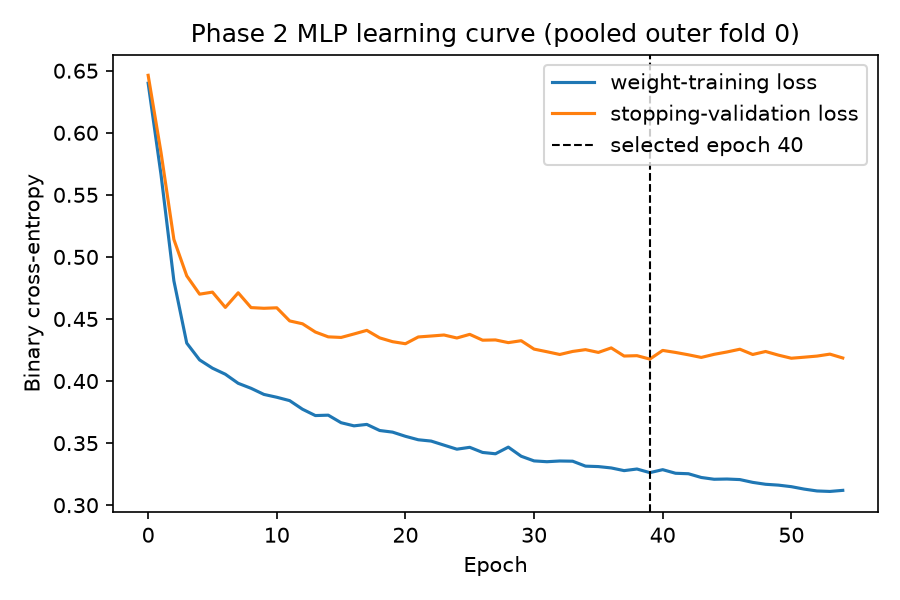
\includegraphics[width=0.92\columnwidth]{mlp_learning_curve.png}
\caption{MLP learning curve (pooled outer fold 0): binary cross-entropy on weight-training and stopping rows. The dashed line marks the restored epoch.}
\label{fig:lc}
\end{figure}

\subsection{Ablation studies (RQ4)}
Table~\ref{tab:ablation} varies one factor at a time. Every MLP variant lies within about 0.003 ROC AUC of the full model, much less than the fold-to-fold SD of 0.014--0.023. Removing dropout, weight decay or early stopping changes neither AUC nor log loss meaningfully, and a single 16-unit hidden layer is as good as two layers (0.892 vs.\ 0.889). With 13 inputs and $\sim$700 training patients per fold, an additive, near-linear model already captures most of the signal (LR is as good as the MLP), so additional depth and explicit regularisation have little to act on. In the integration suite, the learned stack (0.890) is marginally above the MLP (0.889) and the simple average (0.889), and clearly above the BN with untuned smoothing (0.876); the learned combiner has almost the same log loss as the average (0.417), so its weights mainly reproduce averaging on pooled data.

\begin{table}[t]
\caption{Controlled ablations (5-fold CV, fixed settings)}
\label{tab:ablation}
\centering
\scriptsize
\setlength{\tabcolsep}{3pt}
\begin{tabular}{lccc}
\toprule
Variant & ROC AUC (mean $\pm$ SD) & Log loss & Fit (s) \\
\midrule
\multicolumn{4}{l}{\textit{(a) MLP regularisation and depth}} \\
Full MLP (16--8, $p{=}0.3$, wd $10^{-3}$, ES) & 0.889 $\pm$ 0.017 & 0.417 & 2.4 \\
$-$ dropout (p = 0) & 0.891 $\pm$ 0.016 & 0.422 & 1.7 \\
$-$ weight decay (0) & 0.888 $\pm$ 0.014 & 0.422 & 1.5 \\
$-$ early stopping (150 ep.) & 0.892 $\pm$ 0.023 & 0.419 & 2.9 \\
One hidden layer (16) & 0.892 $\pm$ 0.023 & 0.412 & 1.7 \\
\midrule
\multicolumn{4}{l}{\textit{(b) BN--MLP integration}} \\
BN alone & 0.876 $\pm$ 0.027 & 0.474 & 0.1 \\
MLP alone & 0.889 $\pm$ 0.017 & 0.417 & 1.9 \\
Simple average & 0.889 $\pm$ 0.020 & 0.417 & 1.8 \\
Learned stack (cross-fitted) & 0.890 $\pm$ 0.020 & 0.417 & 5.8 \\
\bottomrule
\end{tabular}

\end{table}

\subsection{Explainability and the BN--MLP contrast}
SHAP ranks the MLP's inputs as \code{ca} (mean $|\phi|$ 0.114), \code{cp} (0.111), \code{oldpeak} (0.070), \code{thal} (0.058) and \code{slope} (0.055), consistent with the Phase~1 permutation importance of LR, RF and GB, which put \code{ca}, \code{thal} and \code{cp} first. Fig.~\ref{fig:surf} compares learned risk surfaces. The MLP's risk rises smoothly as maximum heart rate falls and age rises (\code{age}$\times$\code{thalach}), whereas the BN's surface is a $3\times3$ step function created by tertile discretisation. For \code{trestbps}$\times$\code{cp} the BN surface is constant in blood pressure: in the expert DAG, \code{trestbps}'s only neighbour is its parent \code{age}, so once age is observed blood pressure is d-separated from the disease node and cannot affect the BN posterior at all. The MLP instead learns a modest dependence on blood pressure that is strongest for asymptomatic chest pain (\code{cp}$\,=4$). This is the complementarity that motivated the stack: the BN contributes structure and transferability, the MLP continuous interactions. Because the explanations come from a model fitted on all patients and use complete-case rows (mostly Cleveland), they describe that model, not causal effects.

\begin{figure}[t]
\centering
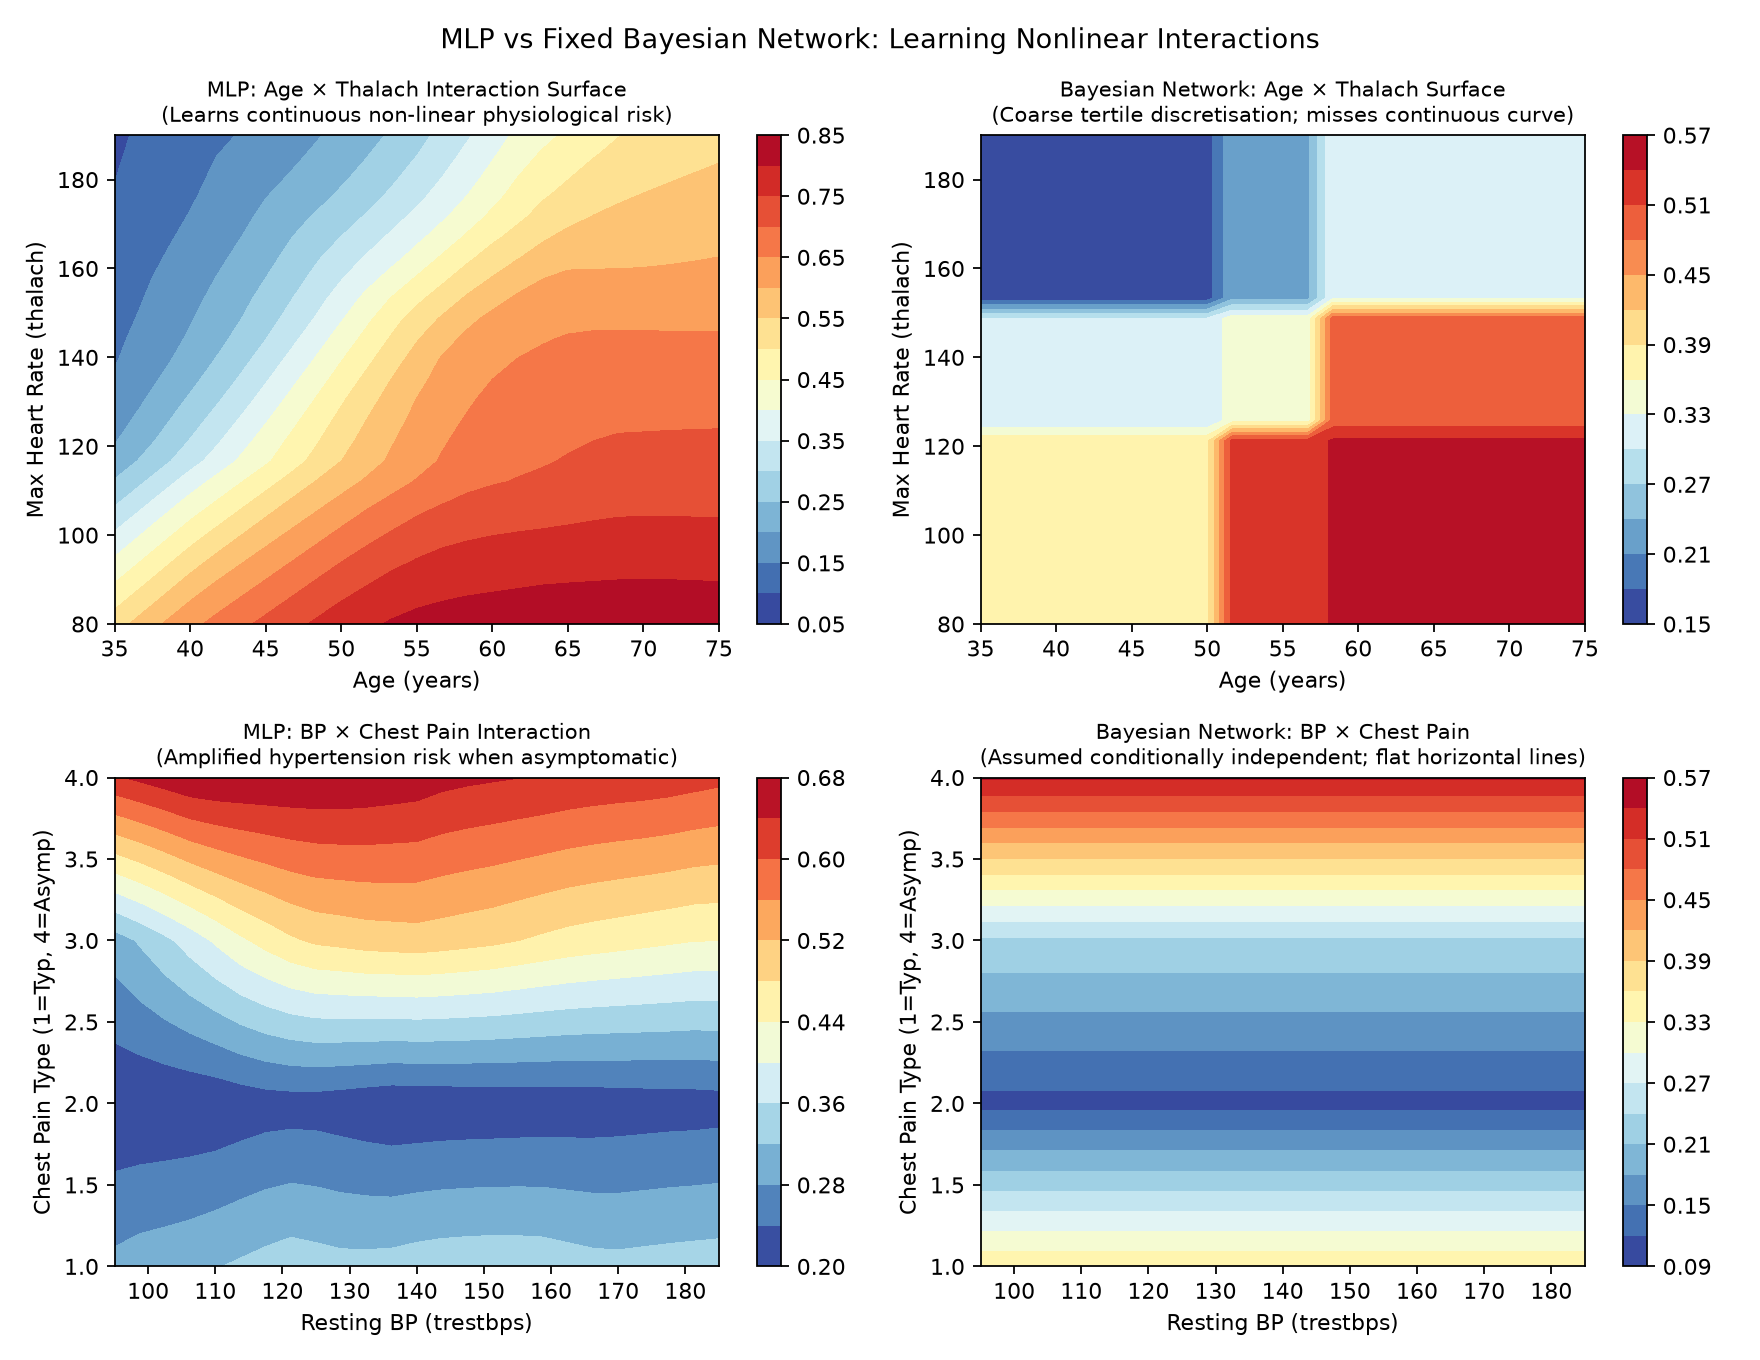
\includegraphics[width=\columnwidth]{mlp_vs_bn_interaction_comparison.png}
\caption{Predicted disease probability over two predictor pairs for the MLP (left) and the BN (right). Only integer values of \code{cp} are meaningful; the contour colouring interpolates between them.}
\label{fig:surf}
\end{figure}

\section{Discussion}
\textbf{RQ1.} Pooling 920 patients does not make the MLP better than LR or the SVM. This agrees with benchmark evidence that neural networks rarely beat well-tuned classical models on small tabular data \cite{grinsztajn,shwartz}; an additive linear model already captures most of the signal, and the ablations confirm there is little nonlinear structure for extra capacity to exploit. \textbf{RQ2.} The cross-fitted stack matches its best constituent on random splits and is significantly better than the MLP when a whole hospital is held out, so integration buys robustness rather than peak accuracy. \textbf{RQ3.} Hospital shift is the dominant effect in this study: switching from random to cohort-held-out validation costs more AUC (0.046--0.079) than the entire spread between models (0.020). The ranking also changes, with the most constrained probabilistic models (NB, BN) transferring best. Random-split results on the UCI data should therefore not be read as evidence about performance at a new site, which is why Detrano \textit{et al.} tested their algorithm across sites \cite{detrano}. \textbf{RQ4.} At this scale, dropout, weight decay, early stopping and a second hidden layer are individually unimportant; the MLP's performance is governed by the data, not the architecture.

Compared with Phase~1, Cleveland AUC within the pooled model is slightly lower (for example BN 0.878 vs.\ 0.910, LR 0.897 vs.\ 0.904). Pooling adds patients but also adds cohorts in which \code{ca} and \code{thal} are mostly imputed, which dilutes the relationships that drive Cleveland predictions. More data from a different distribution is not automatically better.

\section{Limitations and Ethics}
The data are small, old (1980s), referral-based and heterogeneous; prevalence reflects who was sent for angiography, not the population. Imputation by the training mode is a strong simplification for \code{ca}, \code{thal} and \code{slope}, and multiple imputation or missingness indicators should be compared. Switzerland has eight disease-free patients, so its specificity, AUC and calibration are unreliable. The pooled protocol used one repeat of five outer folds and 12 TPE trials per fold, and the trial budget was not varied. The BN structure is an expert assumption, not a learned or causal graph. Several predictors require exercise testing, fluoroscopy or nuclear imaging, so the models do not apply to first-contact screening. No subgroup or fairness analysis was performed, although the cohorts are predominantly male. SHAP values describe the fitted model on complete cases, not causal effects. \textbf{These models are not medical devices and must not be used for clinical decisions;} the web demo states this on every page.

\section{Conclusion and Future Work}
Phase~2 met all four requirements of the Phase~1 feedback: an IEEE report, no hand-written hyperparameter loops (TPE via \code{OptunaSearchCV} for all eight models), all four independent UCI cohorts, and an integrated ML--DL model. Under rigorous nested validation, the regularised MLP and the BN--MLP stack are as accurate and well calibrated as the best classical models but not better. Their value appears under hospital shift, where the stack is significantly more robust than the MLP alone and simple probabilistic models transfer best. Future work: learning the BN structure from data with a missing-state analysis per cohort, multiple imputation, recalibration for a new site's prevalence, more TPE trials and repeated outer folds, and external validation on contemporary data.

\section*{Author Contributions}
\textbf{Vansh Panwar}: Phase~2 foundation (environment, PyTorch/Optuna dependencies, \code{config.phase2.yaml}), BN missing-data handling, the cross-fitted BN--MLP stack and its tests, LOCO splits, Methods and limitations documentation. \textbf{Ayush}: four-cohort loader and verification (hashes, counts, duplicates, missingness), cohort EDA, leakage-safe preprocessing for the larger missingness pattern and the dataset sections. \textbf{K Akshith Kumar}: replacement of the hand-written grid loop by the shared \code{OptunaSearchCV}/TPE builder, search spaces, saved trial histories, the ablation runner and artifact audits. \textbf{Hardik Hathwal}: the sklearn-compatible PyTorch MLP with leakage-safe early stopping, learning curves, the Phase~2 evaluation driver for both protocols, SHAP analysis and the report sources. \textbf{Kabir Sharma}: the Phase~2 web application, offline final-model selection and cached demo fits, and the report-asset audit. All members wrote and reviewed this paper.

\section*{Acknowledgment}
We thank our supervisor, Mr.\ Shobhit Johri, for the Phase~1 feedback that shaped this work, and the original investigators of the UCI Heart Disease data (Cleveland Clinic Foundation, Hungarian Institute of Cardiology, University Hospitals of Zurich and Basel, and V.A. Medical Center, Long Beach).

\bibliographystyle{IEEEtran}
\bibliography{references}

\end{document}
